\documentclass[tikz,border=0pt]{standalone}
\usepackage[utf8]{inputenc}
\usepackage{csquotes}
\usepackage{xcolor}
\usepackage{graphicx}
\usepackage{pgffor}
\usepackage{listings}
\usepackage{array}
\usepackage{fontawesome}
\usepackage{amsmath}

\lstset{
    basicstyle=\ttfamily\fontsize{6}{8}\selectfont,
    breaklines=true,
    % backgroundcolor=\color{black},
    keywordstyle=\color{pink},
    commentstyle=\color{blue},
    stringstyle=\color{white},
    showstringspaces=false,
    frame=none,
    xleftmargin=0.6cm,
    xrightmargin=0.6cm
}

\begin{document}
\begin{tikzpicture}
\useasboundingbox (0,0) rectangle (10.8,10.8);

% Hintergrund in Schwarz
\fill[black] (0,0) rectangle (10.8,10.8);

% Zufällige Einsen und Nullen verteilen
\foreach \i in {1,...,5000} {
    \node[text=green, opacity=0.1, font=\ttfamily\fontsize{5}{6}\selectfont] at (rand*10.8, rand*10.8) {\pgfmathtruncatemacro{\random}{round(rand)}\random};
}

% \fill[red, opacity=0.1] (0.05,5.95) rectangle (10.75,10.75);
% \draw[red, thin] (0.05,5.95) rectangle (10.75,10.75); % 45% Höhe
\node[red, anchor=north west, font=\ttfamily\bfseries\fontsize{8}{9}\selectfont] at (0.1,10.65) {NVD DB Update {\Large{ CVE-2013-3900} - \textbf{Score:}{\Large{ 5.5 }}}};
% % ------------------------------------------------------------------------------------------------------------------------------
% \node[red, anchor=north west, font=\ttfamily\fontsize{8}{9}\selectfont, text width=10.6cm, align=center] at (0.1,10.25) {
% \newline
% \newline
% \newline
% If you want to succeed in penetration testing and cybersecurity, learn at least:
% \newline
% };
% ------------------------------------------------------------------------------------------------------------------------------
\fill[green, opacity=0.1] (0.05,1.15) rectangle (10.75,10.75);
\draw[green, thin] (0.05,1.15) rectangle (10.75,10.75); % 45% Höhe
% \node[green, anchor=north west, font=\ttfamily\bfseries\fontsize{8}{9}\selectfont] at (0.1,5.65) {Solution:};
% ------------------------------------------------------------------------------------------------------------------------------
\node[green, anchor=north west, font=\ttfamily\fontsize{8}{9}\selectfont, text width=10.6cm, align=center] at (0.1,10.25) {
\textbf{Components:}
\begin{scriptsize}
\begin{lstlisting}
 microsoft windows 11 21h2 -
 microsoft windows 10 21h1 -
 microsoft windows 8.1 -
 microsoft windows server 2008 -
 microsoft windows server 2019 -
 microsoft windows server 2008 r2
 microsoft windows server 2012 r2
 microsoft windows 10 21h2 -
 microsoft windows 7 -
 microsoft windows 10 1607 -
 microsoft windows 10 1809 -
 microsoft windows 10 1909 -
 microsoft windows server 2012 -
 microsoft windows 10 1507 -
 microsoft windows server 2022 -
 microsoft windows rt 8.1 -
 microsoft windows server 2016 -
 microsoft windows 10 20h2 -
\end{lstlisting}
\end{scriptsize}
\textbf{Description:}
\begin{scriptsize}
\begin{lstlisting}
Why is Microsoft republishing a CVE from 2013? We are republishing CVE-2013-3900 in the Security Update Guide to update the Security Updates table and to inform customers that the EnableCertPaddingCheck is available in all currently supported versions of Windows 10 and Windows 11. While the format is different from the original CVE published in 2013, except for clarifications about how to configure the EnableCertPaddingCheck registry value, the information herein remains unchanged from the original text published on December 10, 2013, Microsoft does not plan to enforce the stricter verification behavior as a default functionality on supported releases of Microsoft Windows. This behavior remains available as an opt-in feature via reg key setting, and is available on supported editions of Windows released since December 10, 2013. This includes all currently supported versions of Windows 10 and Windows 11. The supporting code for this reg key was incorporated at the time of release for Windows 10 and Windows 11, so no security update is required; however, the reg key must be set. See the Security Updates table for the list of affected software. Vulnerability Description A remote code execution vulnerability exists in the way that the WinVerifyTrust function handles Windows Authenticode signature verification for portable executable (PE) files. An anonymous attacker could exploit the vulnerability by modifying an existing signed executable file to leverage unverified portions of the file in such a way as to add malicious code to the file without invalidating the signature. An attacker who successfully exploited this vulnerability could take complete control of an affected system. An attacker could then install programs; view, change, or delete data; or create new accounts with full user rights. If a user is logged on with administrative user rights, an attacker who successfully exploited this vulnerability could take complete control of an affected system. An attacker could then install programs; view, change, or delete data; or create new accounts with full user rights. Users whose accounts are configured to have fewer user rights on the system could be less impacted than users who operate with administrative user rights. Exploitation of this vulnerability requires that a user or application run or install a specially crafted, signed PE file. An attacker could modify an... See more at https://msrc.microsoft.com/update-guide/vulnerability/CVE-2013-3900
\end{lstlisting}
\end{scriptsize}
\textbf{Main problems:}
\begin{scriptsize}
\begin{lstlisting}
347 "Improper Verification of Cryptographic Signature"

\end{lstlisting}
\end{scriptsize}
};
% ------------------------------------------------------------------------------------------------------------------------------
\draw[green, thin] (0.05,0.05) rectangle (10.75,1.05); % 10% Höhe
% \node[green, anchor=north west, font=\ttfamily\bfseries\fontsize{5}{6}\selectfont] at (0.1,0.95) {Contact:};

% Tabelle 2x2 im Contact Block
\node[green, anchor=north west, font=\ttfamily\fontsize{8}{9}\selectfont, text width=10.6cm] at (0.1,0.95) {
\begin{tabular}{@{}p{4.8cm}@{}p{5cm}@{}}
\faGlobe\ https://cybersword.tech & \faLinkedin\ www.linkedin.com/in/cybersword-tech \\
\faInstagram\ ph1sher & \faTwitter\ @davidwowa \\
\end{tabular}
};
\end{tikzpicture}
\end{document}